\section{Lessons Learned Perspective}
\subsection{Biggest issues}
\subsubsection{Evolution and refactoring}
The main issue we had with the refactoring of the old code was the lack of documentation. A large part of the group had no proficiency with neither Python nor Flask, and we were therefore forced to invest much time into understanding the system. One of the takeaways from this was how difficult it could be to understand and further develop old code when there is a lack of documentation – which is something that often can happen in the real world.

To challenge us as a DevOps team, we decided to also evolve the old software further, by adding new features. Examples of this are the new design and the chat-functionality. Although these functionalities were not the focus, it was a useful learning experience and training in continuous deployment and releasing small features often.

\subsubsection{Maintenance and operation}

Regarding maintenance and operation, one of the largest issues was that we often had some periods with long downtime. For the sake of simplicity, we have narrowed it down to four different major down periods in this report. These are marked with blue (from now on referred to as first), dark blue (from now on referred to as second), yellow (from now on referred to as third), and green (from now on referred to as the last) in figure 1. 

\begin{figure}[h!]
    \centering
    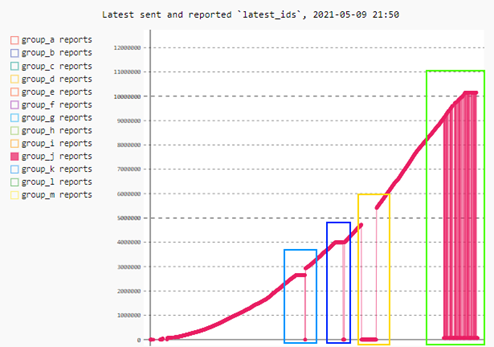
\includegraphics[scale=0.7]{images/downperiodes.png}
    \caption{The graph showing "latest", a int which is updated for each completed job sent from the simulator }
\end{figure}
 
All these different down periods had different solutions, and we have decided to discuss the two down periods we learned the most from, the first down period and the second one. The first down period was due to a crash with our database software (PostgreSQL), and in the second down period, it was due to a crash simulator-side. Although logging helped us out in the last down period, we realized too late that the system was down, resulting in a longer down period. The major lesson learned from the two down periods was that we should have implemented some sort of alerting that would sent to all the team members in case of a failure. This was something we started to implement in Kibana, however, due to lack of time in the end of the simulation, we did not have time to implement it.

\subsubsection{DevOps way of working - CONSIDER REWRITING}

Throughout the project, we as a group have kept the “three ways” characterizing DevOps in mind; flow, feedback, and continual learning and experimentation (REFERENCE TO THE DEVOPS HANDBOOK). Looking at these principles, one of the main differences from other group work is centered around the feedback principle. In earlier projects, we developed tests as a part of the development, but they were rarely executed. This resulted in hours of development, where the newly developed code was not tested, leaving us to scrap non-working code and rewrite it. During this project, after the setup of our pipelines, we have been able to continuously test our project. We have also used tools such as Sonarcloud and CodeQL, which has led us to not only develop better code, but also ensure that the code had enough test-coverage and no security risks before it was deployed. This where the DevOps way of working impacted our work the most, as it was a huge improvement from how we formerly have been thinking about testing.